% ----------------------------------------------------------------
% Compile this file using:
% pdflatex paper
% ----------------------------------------------------------------
\documentclass[utf8,twocolumn]{article}
\usepackage{graphicx,multirow,hyperref,pdfpages}
\begin{document}

\title{A Sample Document With LabPal Data}
\author{Fred Flintstone}
\maketitle

% ----------------------------------------------------------------
% File generated by LabPal 2.7
% Date:     31-01-2017
% Lab name: Sorting Algorithms
%
% To insert one of the tables into your text, do:
% \begin{table}
% \usebox{\boxname}
% \end{table}
% where \boxname is one of the boxes defined in the file below
% ----------------------------------------------------------------

% ----------------------
% Table: sorttime
% ----------------------
\newsavebox{\sorttime}
\begin{lrbox}{\sorttime}
\begin{tabular}{|c|c|c|}
\hline
\textbf{size} & \textbf{time} & \textbf{name}\\
\hline\hline
 \multirow{4}{*}{\href{T1.3.0}{5000}} & {\href{T1.1.1}{0.613001}} & {\href{T1.1.2}{Shell Sort}}\\
\cline{2-3}
 & {\href{T1.0.1}{0.819734}} & {\href{T1.0.2}{Quick Sort}}\\
\cline{2-3}
 & {\href{T1.3.1}{31.731983}} & {\href{T1.3.2}{Gnome Sort}}\\
\cline{2-3}
 & {\href{T1.2.1}{57.07868}} & {\href{T1.2.2}{Bubble Sort}}\\
\hline
 \multirow{4}{*}{\href{T1.5.0}{10000}} & {\href{T1.4.1}{1.560926}} & {\href{T1.4.2}{Quick Sort}}\\
\cline{2-3}
 & {\href{T1.5.1}{2.402894}} & {\href{T1.5.2}{Shell Sort}}\\
\cline{2-3}
 & {\href{T1.7.1}{117.29129}} & {\href{T1.7.2}{Gnome Sort}}\\
\cline{2-3}
 & {\href{T1.6.1}{201.5234}} & {\href{T1.6.2}{Bubble Sort}}\\
\hline
 \multirow{4}{*}{\href{T1.8.0}{15000}} & {\href{T1.8.1}{2.844152}} & {\href{T1.8.2}{Quick Sort}}\\
\cline{2-3}
 & {\href{T1.9.1}{7.868555}} & {\href{T1.9.2}{Shell Sort}}\\
\cline{2-3}
 & {\href{T1.11.1}{266.1354}} & {\href{T1.11.2}{Gnome Sort}}\\
\cline{2-3}
 & {\href{T1.10.1}{505.67435}} & {\href{T1.10.2}{Bubble Sort}}\\
\hline
 \multirow{4}{*}{\href{T1.13.0}{20000}} & {\href{T1.12.1}{4.176307}} & {\href{T1.12.2}{Quick Sort}}\\
\cline{2-3}
 & {\href{T1.13.1}{5.23617}} & {\href{T1.13.2}{Shell Sort}}\\
\cline{2-3}
 & {\href{T1.15.1}{470.69592}} & {\href{T1.15.2}{Gnome Sort}}\\
\cline{2-3}
 & {\href{T1.14.1}{899.84033}} & {\href{T1.14.2}{Bubble Sort}}\\
\hline
 \multirow{4}{*}{\href{T1.19.0}{25000}} & {\href{T1.16.1}{4.215712}} & {\href{T1.16.2}{Quick Sort}}\\
\cline{2-3}
 & {\href{T1.17.1}{6.794177}} & {\href{T1.17.2}{Shell Sort}}\\
\cline{2-3}
 & {\href{T1.19.1}{793.6945}} & {\href{T1.19.2}{Gnome Sort}}\\
\cline{2-3}
 & {\href{T1.18.1}{1408.1387}} & {\href{T1.18.2}{Bubble Sort}}\\
\hline
 \multirow{4}{*}{\href{T1.23.0}{30000}} & {\href{T1.20.1}{8.513943}} & {\href{T1.20.2}{Quick Sort}}\\
\cline{2-3}
 & {\href{T1.21.1}{13.747478}} & {\href{T1.21.2}{Shell Sort}}\\
\cline{2-3}
 & {\href{T1.23.1}{1050.8682}} & {\href{T1.23.2}{Gnome Sort}}\\
\cline{2-3}
 & {\href{T1.22.1}{2025.7166}} & {\href{T1.22.2}{Bubble Sort}}\\
\hline
 \multirow{4}{*}{\href{T1.26.0}{35000}} & {\href{T1.24.1}{4.794233}} & {\href{T1.24.2}{Quick Sort}}\\
\cline{2-3}
 & {\href{T1.25.1}{9.04799}} & {\href{T1.25.2}{Shell Sort}}\\
\cline{2-3}
 & {\href{T1.27.1}{1424.379}} & {\href{T1.27.2}{Gnome Sort}}\\
\cline{2-3}
 & {\href{T1.26.1}{2736.4849}} & {\href{T1.26.2}{Bubble Sort}}\\
\hline
 \multirow{4}{*}{\href{T1.31.0}{40000}} & {\href{T1.28.1}{6.609544}} & {\href{T1.28.2}{Quick Sort}}\\
\cline{2-3}
 & {\href{T1.29.1}{7.226375}} & {\href{T1.29.2}{Shell Sort}}\\
\cline{2-3}
 & {\href{T1.31.1}{1883.648}} & {\href{T1.31.2}{Gnome Sort}}\\
\cline{2-3}
 & {\href{T1.30.1}{3633.834}} & {\href{T1.30.2}{Bubble Sort}}\\
\hline
 \multirow{4}{*}{\href{T1.33.0}{45000}} & {\href{T1.32.1}{4.827898}} & {\href{T1.32.2}{Quick Sort}}\\
\cline{2-3}
 & {\href{T1.33.1}{8.07502}} & {\href{T1.33.2}{Shell Sort}}\\
\cline{2-3}
 & {\href{T1.35.1}{2368.5808}} & {\href{T1.35.2}{Gnome Sort}}\\
\cline{2-3}
 & {\href{T1.34.1}{4570.3594}} & {\href{T1.34.2}{Bubble Sort}}\\
\hline
 \multirow{4}{*}{\href{T1.36.0}{50000}} & {\href{T1.36.1}{5.266864}} & {\href{T1.36.2}{Quick Sort}}\\
\cline{2-3}
 & {\href{T1.37.1}{9.274715}} & {\href{T1.37.2}{Shell Sort}}\\
\cline{2-3}
 & {\href{T1.39.1}{2919.5515}} & {\href{T1.39.2}{Gnome Sort}}\\
\cline{2-3}
 & {\href{T1.38.1}{5669.2163}} & {\href{T1.38.2}{Bubble Sort}}\\
\hline
 \multirow{4}{*}{\href{T1.42.0}{55000}} & {\href{T1.40.1}{6.047056}} & {\href{T1.40.2}{Quick Sort}}\\
\cline{2-3}
 & {\href{T1.41.1}{9.717643}} & {\href{T1.41.2}{Shell Sort}}\\
\cline{2-3}
 & {\href{T1.43.1}{3547.5903}} & {\href{T1.43.2}{Gnome Sort}}\\
\cline{2-3}
 & {\href{T1.42.1}{6847.2227}} & {\href{T1.42.2}{Bubble Sort}}\\
\hline
 \multirow{4}{*}{\href{T1.44.0}{60000}} & {\href{T1.44.1}{6.550205}} & {\href{T1.44.2}{Quick Sort}}\\
\cline{2-3}
 & {\href{T1.45.1}{11.159963}} & {\href{T1.45.2}{Shell Sort}}\\
\cline{2-3}
 & {\href{T1.47.1}{4197.049}} & {\href{T1.47.2}{Gnome Sort}}\\
\cline{2-3}
 & {\href{T1.46.1}{8142.8438}} & {\href{T1.46.2}{Bubble Sort}}\\
\hline
 \multirow{4}{*}{\href{T1.51.0}{65000}} & {\href{T1.48.1}{6.993936}} & {\href{T1.48.2}{Quick Sort}}\\
\cline{2-3}
 & {\href{T1.49.1}{12.06618}} & {\href{T1.49.2}{Shell Sort}}\\
\cline{2-3}
 & {\href{T1.51.1}{4957.2056}} & {\href{T1.51.2}{Gnome Sort}}\\
\cline{2-3}
 & {\href{T1.50.1}{9576.894}} & {\href{T1.50.2}{Bubble Sort}}\\
\hline
 \multirow{4}{*}{\href{T1.52.0}{70000}} & {\href{T1.52.1}{9.978904}} & {\href{T1.52.2}{Quick Sort}}\\
\cline{2-3}
 & {\href{T1.53.1}{13.525684}} & {\href{T1.53.2}{Shell Sort}}\\
\cline{2-3}
 & {\href{T1.55.1}{5750.1978}} & {\href{T1.55.2}{Gnome Sort}}\\
\cline{2-3}
 & {\href{T1.54.1}{11192.245}} & {\href{T1.54.2}{Bubble Sort}}\\
\hline
 \multirow{4}{*}{\href{T1.57.0}{75000}} & {\href{T1.56.1}{8.176735}} & {\href{T1.56.2}{Quick Sort}}\\
\cline{2-3}
 & {\href{T1.57.1}{14.04746}} & {\href{T1.57.2}{Shell Sort}}\\
\cline{2-3}
 & {\href{T1.59.1}{6585.8857}} & {\href{T1.59.2}{Gnome Sort}}\\
\cline{2-3}
 & {\href{T1.58.1}{12758.962}} & {\href{T1.58.2}{Bubble Sort}}\\
\hline
 \multirow{4}{*}{\href{T1.60.0}{80000}} & {\href{T1.60.1}{10.430194}} & {\href{T1.60.2}{Quick Sort}}\\
\cline{2-3}
 & {\href{T1.61.1}{17.678904}} & {\href{T1.61.2}{Shell Sort}}\\
\cline{2-3}
 & {\href{T1.63.1}{8154.84}} & {\href{T1.63.2}{Gnome Sort}}\\
\cline{2-3}
 & {\href{T1.62.1}{13693.364}} & {\href{T1.62.2}{Bubble Sort}}\\

\hline
\end{tabular}
\end{lrbox}

% ----------------------
% Table: sorttimealg
% ----------------------
\newsavebox{\sorttimealg}
\begin{lrbox}{\sorttimealg}
\begin{tabular}{|c|c|c|c|c|}
\hline
\textbf{size} & \textbf{Bubble Sort} & \textbf{Shell Sort} & \textbf{Quick Sort} & \textbf{Gnome Sort}\\
\hline\hline
{\href{T2.0.0}{5000}} & {\href{T2.0.1}{57.07868}} & {\href{T2.0.2}{0.613001}} & {\href{T2.0.3}{0.819734}} & {\href{T2.0.4}{31.731983}}\\
\hline
{\href{T2.1.0}{10000}} & {\href{T2.1.1}{201.5234}} & {\href{T2.1.2}{2.402894}} & {\href{T2.1.3}{1.560926}} & {\href{T2.1.4}{117.29129}}\\
\hline
{\href{T2.2.0}{15000}} & {\href{T2.2.1}{505.67435}} & {\href{T2.2.2}{7.868555}} & {\href{T2.2.3}{2.844152}} & {\href{T2.2.4}{266.1354}}\\
\hline
{\href{T2.3.0}{20000}} & {\href{T2.3.1}{899.84033}} & {\href{T2.3.2}{5.23617}} & {\href{T2.3.3}{4.176307}} & {\href{T2.3.4}{470.69592}}\\
\hline
{\href{T2.4.0}{25000}} & {\href{T2.4.1}{1408.1387}} & {\href{T2.4.2}{6.794177}} & {\href{T2.4.3}{4.215712}} & {\href{T2.4.4}{793.6945}}\\
\hline
{\href{T2.5.0}{30000}} & {\href{T2.5.1}{2025.7166}} & {\href{T2.5.2}{13.747478}} & {\href{T2.5.3}{8.513943}} & {\href{T2.5.4}{1050.8682}}\\
\hline
{\href{T2.6.0}{35000}} & {\href{T2.6.1}{2736.4849}} & {\href{T2.6.2}{9.04799}} & {\href{T2.6.3}{4.794233}} & {\href{T2.6.4}{1424.379}}\\
\hline
{\href{T2.7.0}{40000}} & {\href{T2.7.1}{3633.834}} & {\href{T2.7.2}{7.226375}} & {\href{T2.7.3}{6.609544}} & {\href{T2.7.4}{1883.648}}\\
\hline
{\href{T2.8.0}{45000}} & {\href{T2.8.1}{4570.3594}} & {\href{T2.8.2}{8.07502}} & {\href{T2.8.3}{4.827898}} & {\href{T2.8.4}{2368.5808}}\\
\hline
{\href{T2.9.0}{50000}} & {\href{T2.9.1}{5669.2163}} & {\href{T2.9.2}{9.274715}} & {\href{T2.9.3}{5.266864}} & {\href{T2.9.4}{2919.5515}}\\
\hline
{\href{T2.10.0}{55000}} & {\href{T2.10.1}{6847.2227}} & {\href{T2.10.2}{9.717643}} & {\href{T2.10.3}{6.047056}} & {\href{T2.10.4}{3547.5903}}\\
\hline
{\href{T2.11.0}{60000}} & {\href{T2.11.1}{8142.8438}} & {\href{T2.11.2}{11.159963}} & {\href{T2.11.3}{6.550205}} & {\href{T2.11.4}{4197.049}}\\
\hline
{\href{T2.12.0}{65000}} & {\href{T2.12.1}{9576.894}} & {\href{T2.12.2}{12.06618}} & {\href{T2.12.3}{6.993936}} & {\href{T2.12.4}{4957.2056}}\\
\hline
{\href{T2.13.0}{70000}} & {\href{T2.13.1}{11192.245}} & {\href{T2.13.2}{13.525684}} & {\href{T2.13.3}{9.978904}} & {\href{T2.13.4}{5750.1978}}\\
\hline
{\href{T2.14.0}{75000}} & {\href{T2.14.1}{12758.962}} & {\href{T2.14.2}{14.04746}} & {\href{T2.14.3}{8.176735}} & {\href{T2.14.4}{6585.8857}}\\
\hline
{\href{T2.15.0}{80000}} & {\href{T2.15.1}{13693.364}} & {\href{T2.15.2}{17.678904}} & {\href{T2.15.3}{10.430194}} & {\href{T2.15.4}{8154.84}}\\

\hline
\end{tabular}
\end{lrbox}

% ----------------------
% Table: sumtime
% ----------------------
\newsavebox{\sumtime}
\begin{lrbox}{\sumtime}
\begin{tabular}{|c|c|c|c|c|}
\hline
\textbf{size} & \textbf{Bubble Sort} & \textbf{Shell Sort} & \textbf{Quick Sort} & \textbf{Gnome Sort}\\
\hline\hline
{\href{T3.0.0}{680000.0}} & {\href{T3.0.1}{83919.41}} & {\href{T3.0.2}{148.48221}} & {\href{T3.0.3}{91.806335}} & {\href{T3.0.4}{44519.344}}\\

\hline
\end{tabular}
\end{lrbox}


% ----------------------------------------------------------------
% File generated by LabPal 2.7
% Date:     31-01-2017
% Lab name: Sorting Algorithms
%
% To insert one of the figures into your text, do:
% \begin{figure}
% \usebox{\boxname}
% \end{figure}
% where \boxname is one of the boxes defined in the file below
% ----------------------------------------------------------------

% ----------------------
% Plot: sortplot
% ----------------------
\newsavebox{\sortplot}
\begin{lrbox}{\sortplot}
\href{P1.0}{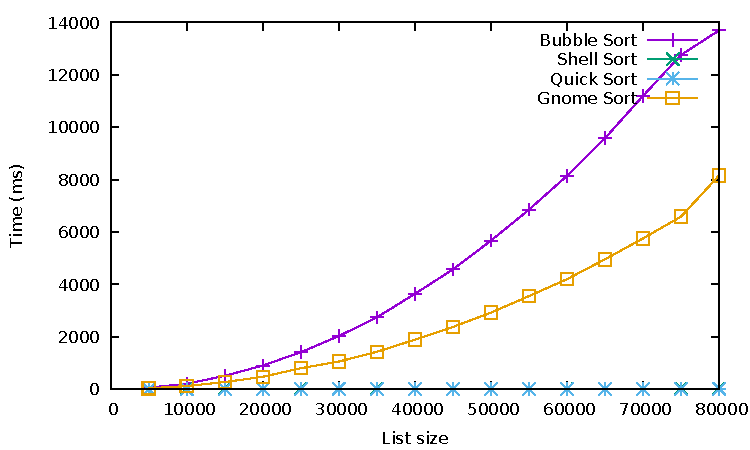
\includegraphics[page=1,width=\linewidth]{labpal-plots.pdf}}
\end{lrbox}

% ----------------------
% Plot: sorthisto
% ----------------------
\newsavebox{\sorthisto}
\begin{lrbox}{\sorthisto}
\href{P2.0}{\includegraphics[page=2,width=\linewidth]{labpal-plots.pdf}}
\end{lrbox}

% ----------------------
% Plot: plotsumtime
% ----------------------
\newsavebox{\plotsumtime}
\begin{lrbox}{\plotsumtime}
\href{P3.0}{\includegraphics[page=3,width=\linewidth]{labpal-plots.pdf}}
\end{lrbox}


% ----------------------------------------------------------------
% File generated by LabPal 2.7
% Date:     31-01-2017
% Lab name: Sorting Algorithms
% ----------------------------------------------------------------

% maxSize
% The maximum size of the arrays sorted in the experiments
\newcommand{\maxSize}{\href{M1.0}{80000}}

% numAlgos
% The number of algorithms compared in this lab
\newcommand{\numAlgos}{\href{M2.0}{4}}

% slowestAlgo
% The name of the slowest sorting algorithm
\newcommand{\slowestAlgo}{\href{M3.0}{Bubble Sort}}



This is a simple \LaTeX{} document showing how to include plots, macros and
tables generated with LabPal inside your research paper. Our paper will use the
data generated by the \emph{Sorting Lab} example contained in LabPal's example
folder.

\section*{Required Packages}

Make sure your \LaTeX{} file imports the following packages:

\begin{itemize}
\item \texttt{graphicx} and \texttt{pdfpages} to include figures
\item \texttt{multirow} for tables
\item \texttt{hyperref} for the hyperlink functionalities
\end{itemize}

\section*{Importing the Files}

The first step is to run the experiments in the lab, and to export four files:

\begin{itemize}
\item The PDF files for all plots in the lab. Go to the \textsl{Plots} page and
click on the ``Download all plots'' button. By default, the file is called
\verb+labpal-plots.pdf+.
\item The macro file to easily import the plots. In the \textsl{Plots} page,
click on the ``Download \LaTeX{} macros'' button. By default, the file is called
\verb+labpal-plots.tex+.
\item The \LaTeX{} file for the tables. In the \textsl{Tables} page, click on
the ``Download all tables'' button. By default, the file is called
\verb+labpal-tables.tex+.
\item The \LaTeX{} file for the macros. In the \textsl{Macros} page, click on
the ``Download all macros'' button. By default, the file is called
\verb+labpal-macros.tex+.
\end{itemize}

Copy these files in the same folder as your research paper. At the top of the
paper, make sure you include the two \texttt{.tex} files using the
\texttt{input} command.

\section*{Adding a Table}

To add a table to your text, create a \texttt{table} environment as usual. Use
the command \verb+\usebox{\boxname}+ to include the contents of a table, where
\verb+boxname+ is the name of one of the boxes defined in
\verb+labpal-tables.tex+. (In your lab, you can set the name given to each
table's box through method \verb+setNickname()+. Otherwise, LabPal assigns a
default name to each table.)

\begin{table}
\centering
\usebox{\sorttime}
\caption{This table is generated by LabPal. Hyperlinks in the table refer to
individual data points in the lab.}
\label{table-sort}
\end{table}

Table \ref{table-sort} shows an example of a table included in such a way. Each
cell in the table is a hyperlink. The destination of each link can be
copy-pasted in LabPal's web console, in the \textsl{Find} page, which takes you
to the table, plot or macro where this specific data point is defined.

\section*{Adding a Plot}

Adding a plot can be done in the same way as a table; create a \texttt{figure}
environment, and use the \verb+\usebox{\boxname}+ to include a specific image;
\verb+boxname+ is the name of one of the boxes defined in
\verb+labpal-plots.tex+.

\begin{figure}
\centering
\usebox{\sortplot}
\caption{This plot is generated by LabPal. The hyperlink points to the same
figure inside the lab instance.}
\end{figure}

Figure \ref{table-sort} shows an example of a figure included in such a way. The
figure is surrounded by a hyperlink. The destination of this link can be
copy-pasted in LabPal's web console, in the \textsl{Find} page, which takes you
to the plot and its associated data table.

\section*{Referring to Macros}

Referring to macros is even easier. Simply call any of the commands defined in
\verb+labpal-macros.tex+ wherever in the text. For example, we know that the
slowest sorting algorithm is \slowestAlgo{}, and that our lab has considered
arrays of size up to \maxSize{}.

\end{document}